\subsection{Encoder depth is task-dependent}
\label{sec:res_depth}

All results in this section use the \textsc{disjoint} reference protocol of
Section~\ref{sec:refproto} at $N = 500$, so the cohort effects of
Section~\ref{sec:res_cohort} are controlled. Table~\ref{tab:depthgrid} and
Fig.~\ref{fig:depthgrid} summarise every task at every block.

\paragraph{Fidelity peaks before the final block}
Permutation $z$ for the real-versus-DDPM comparison rises steeply through the
early blocks, plateaus over \Lb{7}--\Lb{9}, and then declines. The maximum is at
\Lb{8} ($z = 439.3$), with \Lb{7} ($436.9$) and \Lb{9} ($436.6$) statistically
indistinguishable from it. The final block gives $z = 342.4$, which is $22.1\%$
below the plateau. Reading the last layer, the default in work that uses a
foundation model as a metric backbone, therefore discards roughly a fifth of the
available discriminability on this comparison.

The raw discrepancies tell the same story: $\widehat{\mmd}^2$ against the DDPM
is $0.1042$ at \Lb{7} and $0.0732$ at \Lb{12}, while the real-versus-real null
is $\le 0.0003$ at every block. The decline into the final blocks is a loss of
signal, not a change of scale.

Severity ordering, by contrast, is depth-robust. Every one of the twelve blocks
recovers the a-priori ordering
$\text{real} < \text{DDPM} < \text{WDM-3D} < \text{CT} < \text{retinal}$ with
Spearman $\rho = +1.000$. If the only requirement is to rank generators of
clearly different quality, depth does not matter; if the requirement is to
resolve two similar generators, it does.

\paragraph{Near-duplicate detection improves with depth}
Memorization recovery error falls essentially monotonically with depth
(Table~\ref{tab:depthgrid}, second column): mean absolute error is $0.512$ at
\Lb{1}, $0.027$ at \Lb{6}, $0.007$ at \Lb{9} and $0.004$ at \Lb{10}--\Lb{11}.
Shallow blocks are not merely worse, they are unusable: at \Lb{1} the detector
recovers essentially none of the injected duplicates. The behaviour is stable
across jitter scales up to $\sigma = 0.02$ and collapses for all depths at
$\sigma \ge 0.1$, where the perturbation has destroyed the near-duplicate
relationship the detector is meant to find.

This result contradicts an earlier analysis of ours conducted on a
\textsc{head} reference, which reported that shallow blocks outperformed
mid-depth ones for this task. That conclusion was an artefact of the
$17$-subject reference: when the reference spans few subjects, its
within-reference nearest-neighbour distances are small, the detection threshold
is correspondingly tight, and the ranking across depths inverts. We report this
explicitly because it is a concrete instance of the paper's general point ---
the reference protocol changed the sign of a methodological conclusion, not
merely the value of a number.

\paragraph{Degradation monotonicity fails only at the shallowest blocks}
Under a Gaussian noise ladder, $\widehat{\mmd}^2$ increases monotonically with
$\sigma$ at every block from \Lb{3} onwards ($\rho = +1.000$). \Lb{1}
($\rho = +0.857$) and \Lb{2} ($\rho = +0.893$) are non-monotone: mild noise
initially \emph{decreases} the measured discrepancy, because at those depths the
representation is dominated by low-level texture statistics that noise makes
more similar between the two sets before it makes them different. A metric read
at \Lb{1} would report that a slightly corrupted generator had improved.

\begin{table}[t]
\centering
\caption{Depth $\times$ task grid for RadioDINO-s16, $N = 500$, patient-disjoint
reference. Best value per column in bold; the a-priori choice for each task is
marked $\dagger$. No single depth wins every task, and the final block wins
none.}
\label{tab:depthgrid}
\small
\begin{tabular}{rccccc}
\toprule
& Fidelity & Memorization & Coverage & \multicolumn{2}{c}{Per-image AUC} \\
\cmidrule(lr){5-6}
Block & $z_{\mathrm{perm}}$ $\uparrow$ & MAE $\downarrow$
      & $\rho(d,\text{recall})$ $\downarrow$ & centroid & Mahalanobis \\
\midrule
\Lb{1}  & $171.6$ & $0.512$ & $+0.900$ & $0.592$ & $0.461$ \\
\Lb{2}  & $212.6$ & $0.163$ & $+1.000$ & $0.664$ & $0.725$ \\
\Lb{3}  & $185.0$ & $0.180$ & $+1.000$ & $0.646$ & $0.622$ \\
\Lb{4}  & $221.1$ & $0.114$ & $+0.900^{\dagger}$ & $0.654$ & $0.771$ \\
\Lb{5}  & $267.4$ & $0.083$ & $+1.000$ & $0.628$ & $0.858$ \\
\Lb{6}  & $326.5$ & $0.027$ & $+0.900$ & $0.674$ & $0.921$ \\
\Lb{7}  & $436.9$ & $0.013$ & $+1.000$ & $0.744$ & $0.928$ \\
\Lb{8}  & $\mathbf{439.3}$ & $0.016$ & $+0.900$ & $0.796$ & $0.949$ \\
\Lb{9}  & $436.6$ & $0.007^{\dagger}$ & $+0.975$ & $\mathbf{0.846}$ & $\mathbf{0.972}$ \\
\Lb{10} & $404.6$ & $\mathbf{0.004}$ & $+1.000$ & $0.840$ & $\mathbf{0.972}$ \\
\Lb{11} & $368.6$ & $\mathbf{0.004}$ & $+1.000$ & $0.821$ & $0.967$ \\
\Lb{12} & $342.4^{\dagger}$ & $0.008$ & $+0.821$ & $0.810$ & $0.962$ \\
\midrule
Best block & \Lb{8} & \Lb{10}--\Lb{11} & none & \Lb{9} & \Lb{9}--\Lb{10} \\
\bottomrule
\end{tabular}
\end{table}

\begin{figure}[t]
\centering
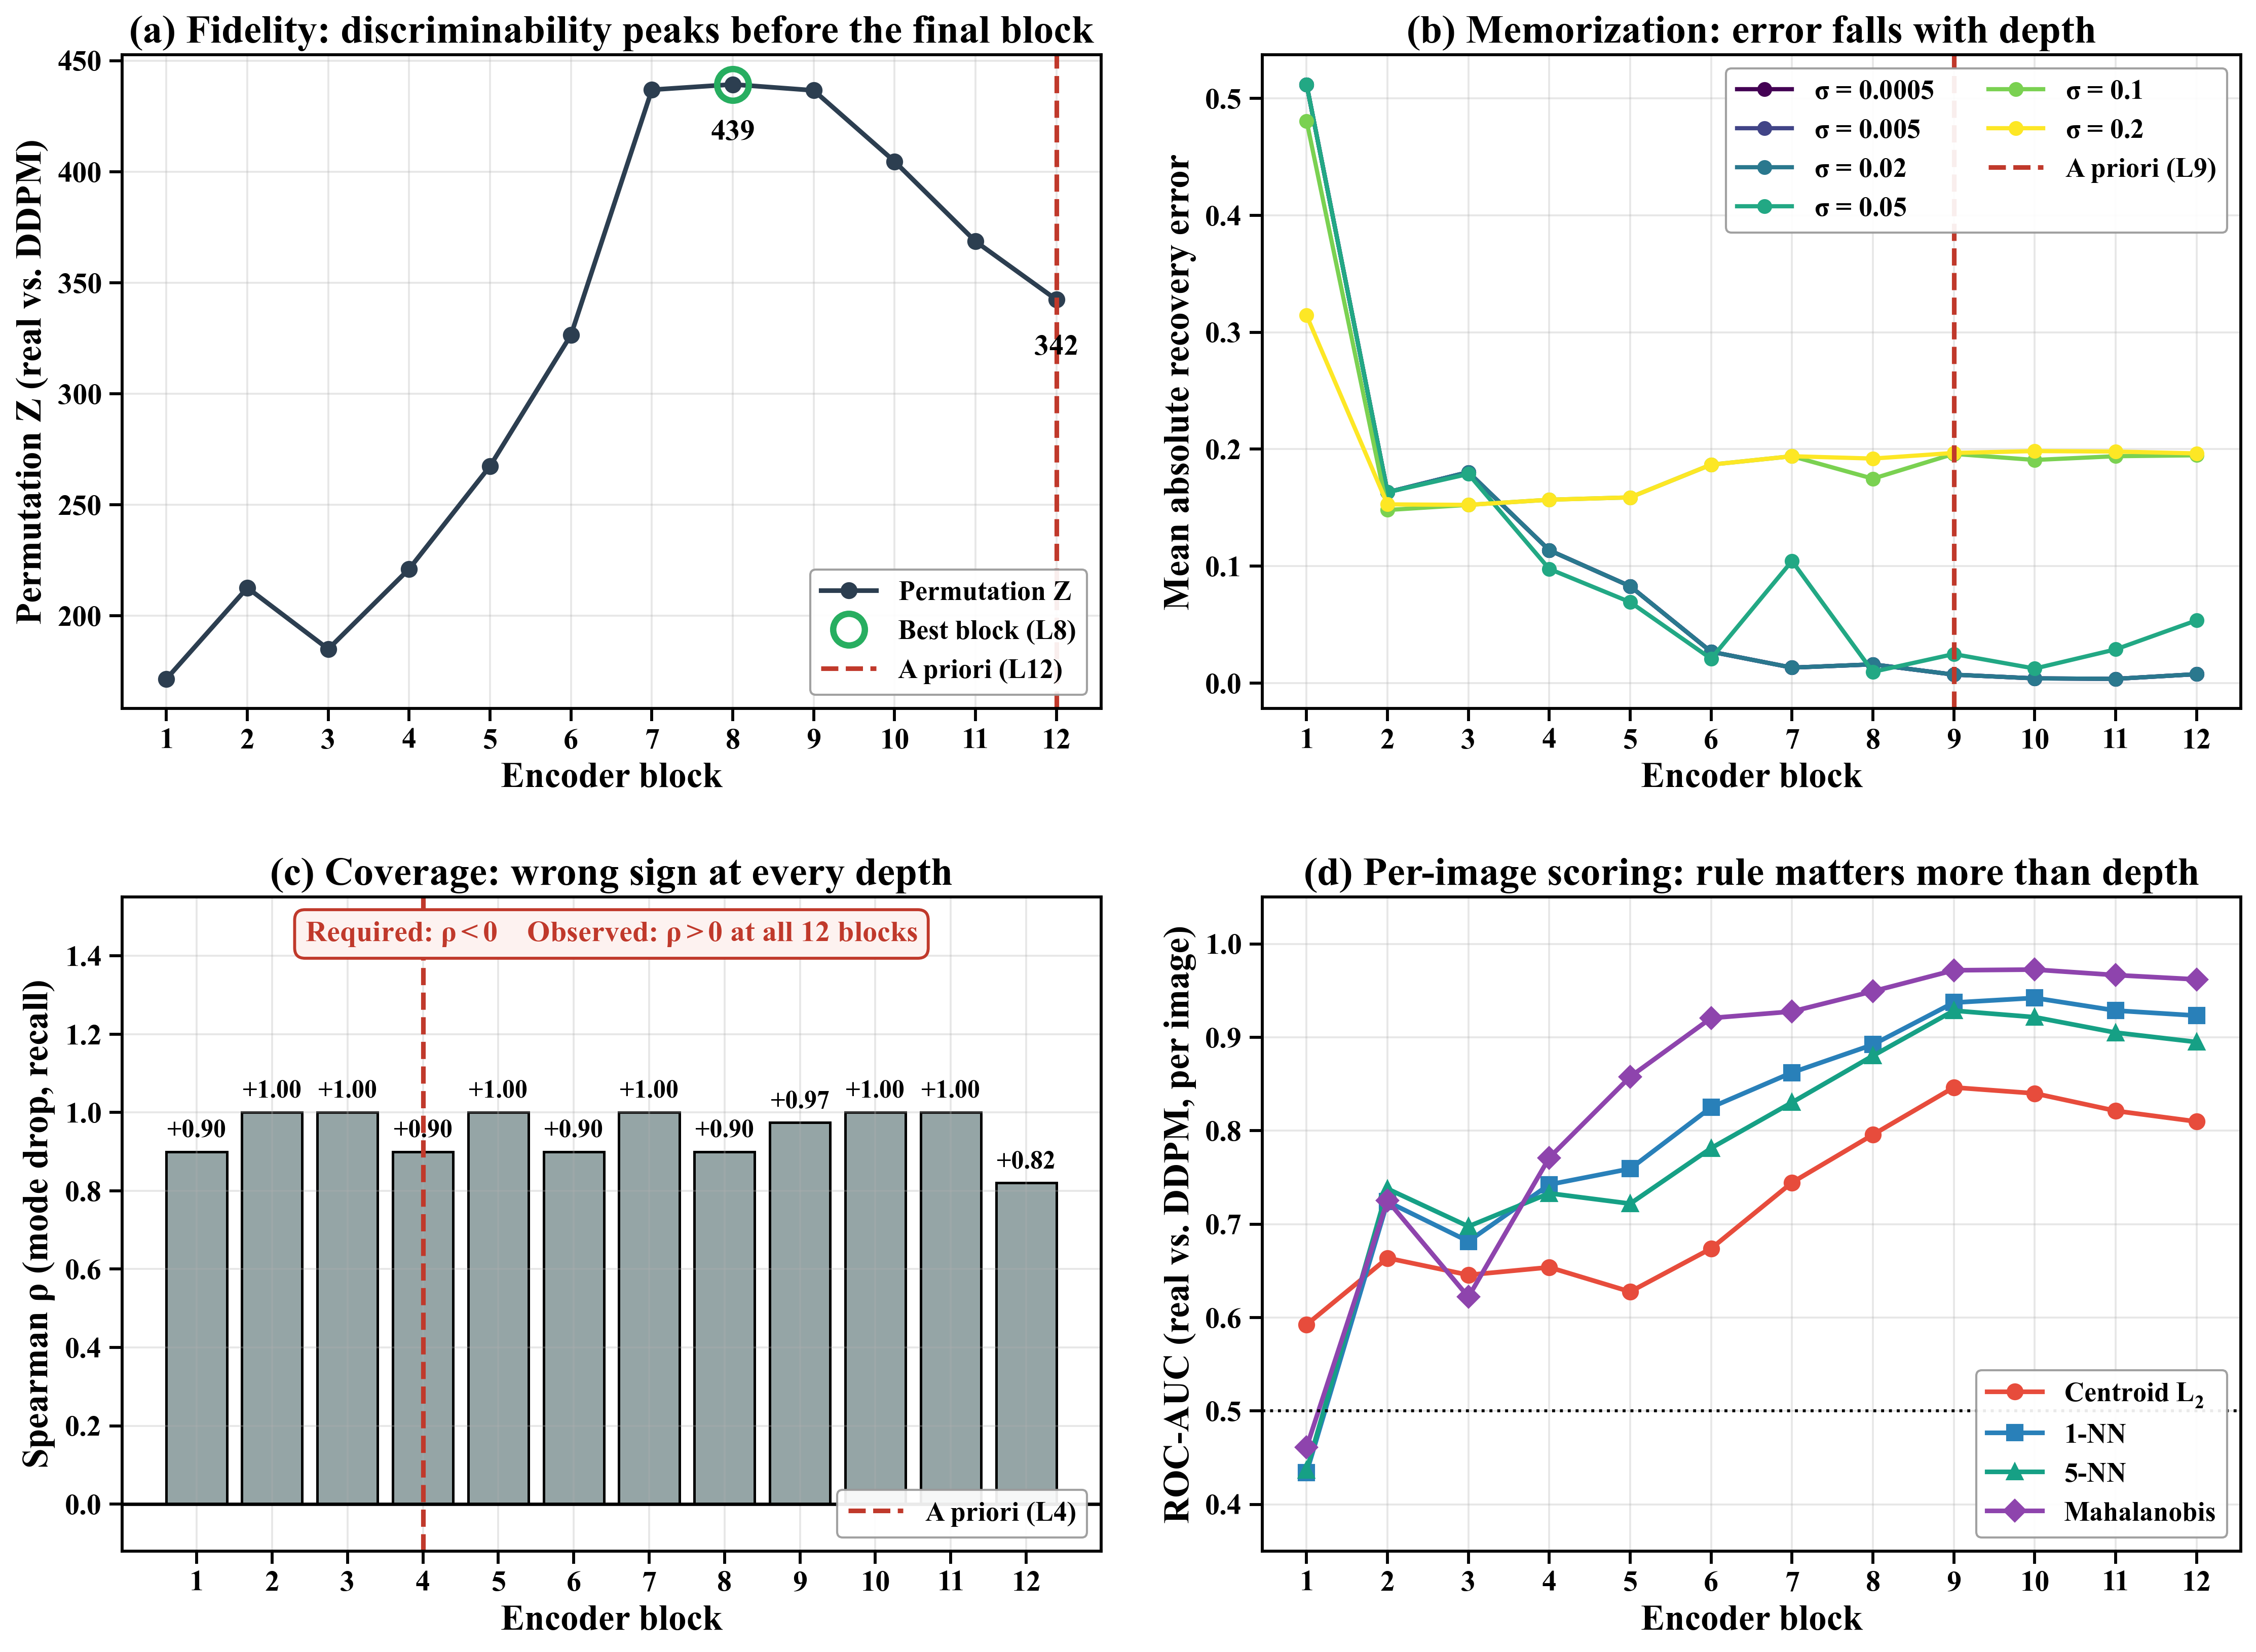
\includegraphics[width=\linewidth]{Images/depth_task_grid.png}
\caption{Depth profiles for four evaluation tasks. (a) Fidelity
discriminability peaks at \Lb{7}--\Lb{9}, not at the final block. (b)
Memorization recovery error falls with depth; curves are jitter scales, and the
task collapses for all depths at large $\sigma$. (c) $k$-NN coverage: the
Spearman correlation between mode drop and recall is positive at every depth,
the opposite of the required sign. (d) Per-image scoring: the choice of
distance separates the curves more than depth does. Dashed vertical lines mark
the a-priori depth for each task.}
\label{fig:depthgrid}
\end{figure}

\subsection{$k$-NN coverage is invalid at every depth}
\label{sec:res_coverage}

The mode-drop validation asks a minimal question: if diversity is deliberately
removed from the generated set, does measured coverage fall? For $k$-NN recall
\citep{kynkaanniemi2019pr} in this feature space, the answer is no at
every one of the twelve blocks. The Spearman correlation between drop fraction
and recall is \emph{positive} everywhere, ranging from $+0.821$ at \Lb{12} to
$+1.000$ at five blocks (Table~\ref{tab:depthgrid}, third column). Discarding
$80\%$ of the generated samples \emph{increases} measured recall --- at \Lb{9},
from $0.008$ to $0.114$.

The mechanism is visible in the raw values and is a known property of the
estimator rather than a pathology of the encoder. Recall is the fraction of real
points falling inside the union of $k$-NN balls around generated points, and
each ball's radius is that point's own $k$-th nearest-neighbour distance
\emph{within the generated set}. Removing generated samples increases every
surviving point's $k$-NN radius, inflating each ball. Below some density the
inflation of the balls outpaces the loss of centres, and measured coverage
rises. In a $384$-dimensional self-supervised embedding, where the generated set
occupies a thin region and absolute recall is already very low ($0.008$--$0.044$
at $d = 0$ for blocks \Lb{7}--\Lb{12}), the estimator is in that regime from the
start.

We therefore report no coverage number in this feature space and recommend that
others do not either without first running this validation. We note that the
diagnostic may behave correctly in embeddings where the generated set is denser
relative to the real manifold; the claim here is specific to the setting, not a
general refutation of the estimator.

\subsection{Per-image scoring depends more on the distance than on the depth}
\label{sec:res_perimage}

Two per-image tasks were run: separating held-out real slices from
cross-modality CT, and separating them from the DDPM's own output. The first is
saturated --- every rule at every depth achieves AUC $\ge 0.997$ --- and is
therefore useless for comparing rules or depths. We note this because
cross-modality OOD detection is a common headline experiment in this
literature, and a saturated benchmark cannot support the conclusions usually
drawn from it.

On the discriminative same-modality task, the ranking of rules is consistent
across depth and larger than the effect of depth itself
(Table~\ref{tab:depthgrid}, last two columns). At the best depth, shrinkage
Mahalanobis reaches AUC $0.972$, $1$-NN $0.942$, $5$-NN $0.929$, and distance to
the reference centroid $0.846$. The centroid rule is worst at every block from
\Lb{2} onward, by a margin of $9$--$23$ AUC points. This is expected on
geometric grounds: a centroid distance assumes an isotropic, unimodal reference,
whereas a medical cohort is neither, and a shrinkage Mahalanobis distance
accounts for the anisotropy that the raw Euclidean distance ignores. Where a
per-image score is required --- for flagging individual synthetic images before
clinical use, for instance --- the distance should be chosen deliberately rather
than defaulted to a centroid.
